\subsection{Benchmark of the calibrator}\label{sec:val-benchmark}
% src: sources/RESULTS_MAP.md section B; tables/coverage_tables.py; figures/fig_coverage.py

\paragraph{Design.} We tested the calibrator on a library of simulated cohorts (library v6) that the SR model itself
generates: each cohort is a sample from Eq.~\eqref{eq:sr} at known parameters, so the benchmark measures
self-recovery and nothing else (Section~\ref{sec:limitations}). The library, every stored per-cohort record, the reports and an interactive explorer of the
results are released with this paper (SI Section~\ref{si:records}; Code and data availability), so that each number
below can be recomputed and any cohort inspected. The library holds \C{v6-n-cohorts} cohorts in six
\emph{arms}: \emph{pure} (homogeneous SR, no censoring; \C{v6-arm-pure} cohorts), \emph{censor} (a fraction of
individuals right-censored; \C{v6-arm-censor}), \emph{hazard} (an added age-independent external hazard;
\C{v6-arm-hazard}), \emph{window} (deaths observed only inside an age window; \C{v6-arm-window}), \emph{het} (a spread
of thresholds $\xc$ across individuals; \C{v6-arm-het}) and \emph{realfull} (simulated at the fitted parameters, sample
size and censoring of real data sets; \C{v6-arm-realfull}). The cohorts fall in four \emph{groups}: main
(\C{v6-group-main}), big-$n$ (\C{v6-group-bign}), sharp, i.e.\ tightly clustered death ages (\C{v6-group-sharp}), and an
$n$-ladder of pure cohorts at fixed $\delta/L$ and graded $n$ (\C{v6-group-nladder}). Truth parameters are laid out on a grid of
\C{v6-kappa-n} values of $\kappa$ from \C{v6-kappa-min} to \C{v6-kappa-max}, crossed with combinations of $\eta$, $\beta$ and $\eps$ that span a range of production-to-removal ratios; sample sizes run from $n=\C{v6-n-min}$ to $n=\C{v6-n-max}$ and the recording interval relative to
the lifespan scale, $\delta/L$, from \C{v6-dL-min} to \C{v6-dL-max}. The full arm-by-group design is in
Table~\ref{tab:library-design} (SI).

A validity audit flags cohorts in which some death has zero probability mass at the SR-only truth on the fit grid:
for arms generated with something the SR-only truth does not contain (an external hazard, a threshold spread) this
happens by construction, so such cohorts are kept but not scored as coverage claims. The audit flagged \C{v6-validity-invalid} of the
\C{v6-validity-rows} cohorts (\C{v6-validity-invalid-pct}\,\%). The reference run of the calibrator covers the main
and big-$n$ groups, \C{gate-v6-n} cohorts (pure \C{d2a-ref-pure}, hazard, window, het and censor \C{d2a-ref-hazard} each,
realfull \C{d2a-ref-realfull}), of which \C{d2a-ref-invalid} are flagged invalid; the flagged cohorts are in the hazard,
het and realfull arms, the arms with a feature the SR-only truth lacks. Sharp and $n$-ladder cohorts are reported separately. Every coverage figure below states its
population and its denominator, the number of cohorts for which a closed interval was claimed.

\paragraph{Scoring.} A fit returns for each of $\eta$, $\beta$, $\eps$, $\kappa$ a claim of one of three shapes: a
closed interval (a \emph{value}), a one-sided \emph{bound}, or \emph{no claim} (Section~\ref{sec:estimation}). We
score each against the truth that generated the cohort. \emph{Closed coverage} is the fraction of closed 95\,\%
intervals that contain the truth, among cohorts with a closed claim; it is conditional on a claim being made, and the
decline rate (share of cohorts with no claim) is reported beside it. One-sided bounds are scored separately.
Binomial uncertainty is a Wilson 95\,\% interval \citep{wilson1927probable}. We also report the median closed width
in decades (dex, $\log_{10}$ units) and the median signed $\log_{10}$ error of the point estimate (bias). Coverage
alone can be bought with width: a data-ignoring \emph{null prior}, which always returns the whole search range,
covers the truth in every cohort (closed $\eta$ coverage \C{v6-null-eta-cov}). Widths and decline rates therefore carry
the information about how much a method learned, and coverage must be read together with them. The release gate
(GATE-V6) has five parts: G1, no arm loses calibration against the previous version; G2, no more truth-witnessed
maximum-likelihood failures than the previous version; G3, pure-arm availability and accuracy no worse; G4, the
diagnostic registry (\C{gate-v6-registry-passed} passed, \C{gate-v6-registry-warned} warned,
\C{gate-v6-registry-failed} failed); G5, integrity of the stored records. All five passed on the reference run
(Table~\ref{tab:gates}, SI).

\paragraph{Coverage on well-specified data.} On the pure arm J's closed 95\,\% intervals contained the truth for
$\eta$ in \C{v6-pure-eta-J-hits} of \C{v6-pure-eta-J-n} cohorts (\C{v6-pure-eta-J}; Wilson \C{d2a-pure-J-eta-wilson_lo}--\C{d2a-pure-J-eta-wilson_hi}), for
$\eps$ in \C{d2a-pure-J-epsilon-hits} of \C{d2a-pure-J-epsilon-n_closed} (\C{v6-pure-eps-J}) and for $\beta$ in
\C{v6-pure-beta-J-hits} of \C{v6-pure-beta-J-n} (\C{v6-pure-beta-J}); H gave \C{v6-pure-eta-H}, \C{d2a-pure-H-epsilon-coverage} and
\C{d2a-pure-H-beta-coverage} (Table~\ref{tab:coverage-main}, Figure~\ref{fig:coverage}A). The censor arm is equally
close to nominal (J $\eta$ \C{v6-censor-eta-J}, H \C{v6-censor-eta-H}). Median closed widths on the pure arm are
\C{d2a-pure-J-eta-median_width_dex} dex for $\eta$ and \C{d2a-pure-J-epsilon-median_width_dex} dex for $\eps$, with a
median signed error of \C{d2a-pure-J-eta-bias_log10} and \C{d2a-pure-J-epsilon-bias_log10} dex. Raw $\beta$ is the weak
quantity: its closed intervals are few (\C{v6-pure-beta-J-n} of \C{d2a-ref-pure} cohorts) and wide (median
\C{d2a-pure-J-beta-median_width_dex} dex), because $\beta$ is tied to the unidentified $\kappa$
(Section~\ref{sec:identifiability}). H declines $\beta$ more often than J (decline rate \C{d2a-pure-H-beta-decline_rate}
against \C{d2a-pure-J-beta-decline_rate} on the pure arm), so its $\beta$ coverage is computed on fewer cohorts and is not
comparable one-to-one.

\begin{table}[t]
\centering\small
\resizebox{\textwidth}{!}{\begin{tabular}{lcccccc}
\toprule
 & \multicolumn{3}{c}{J} & \multicolumn{3}{c}{H} \\
\cmidrule(lr){2-4}\cmidrule(lr){5-7}
Arm & $\eta$ & $\beta$ & $\varepsilon$ & $\eta$ & $\beta$ & $\varepsilon$ \\
\midrule
pure & 0.958 (617/644) & 0.968 (272/281) & 0.959 (627/654) & 0.953 (594/623) & 0.970 (263/271) & 0.956 (609/637) \\
censor & 0.975 (194/199) & 0.927 (38/41) & 0.975 (196/201) & 0.954 (188/197) & 0.907 (39/43) & 0.952 (179/188) \\
hazard & 0.076 (18/237) & 0.286 (2/7) & 0.053 (11/209) & 1.000 (178/178) & 1.000 (20/20) & 0.994 (170/171) \\
window & 0.553 (130/235) & 0.873 (48/55) & 0.329 (77/234) & 1.000 (181/181) & 1.000 (17/17) & 1.000 (173/173) \\
het & 0.159 (37/233) & 0.096 (13/135) & 0.057 (13/230) & 0.171 (36/211) & 0.145 (24/166) & 0.089 (18/203) \\
realfull & 0.439 (54/123) & 0.792 (42/53) & 0.366 (41/112) & 0.954 (83/87) & 1.000 (26/26) & 0.968 (61/63) \\
\bottomrule
\end{tabular}
}
\caption{Closed-interval coverage of the truth (hits/cohorts with a closed claim) by arm, for the calibrator J and its
external-hazard variant H, on the reference run (main and big-$n$ groups, \C{gate-v6-n} cohorts). Nominal level 0.95.
Wilson intervals, medians of width and bias, and decline rates are in Table~\ref{tab:coverage-full} (SI).}
\label{tab:coverage-main}
\end{table}

\begin{figure}[t]
\centering
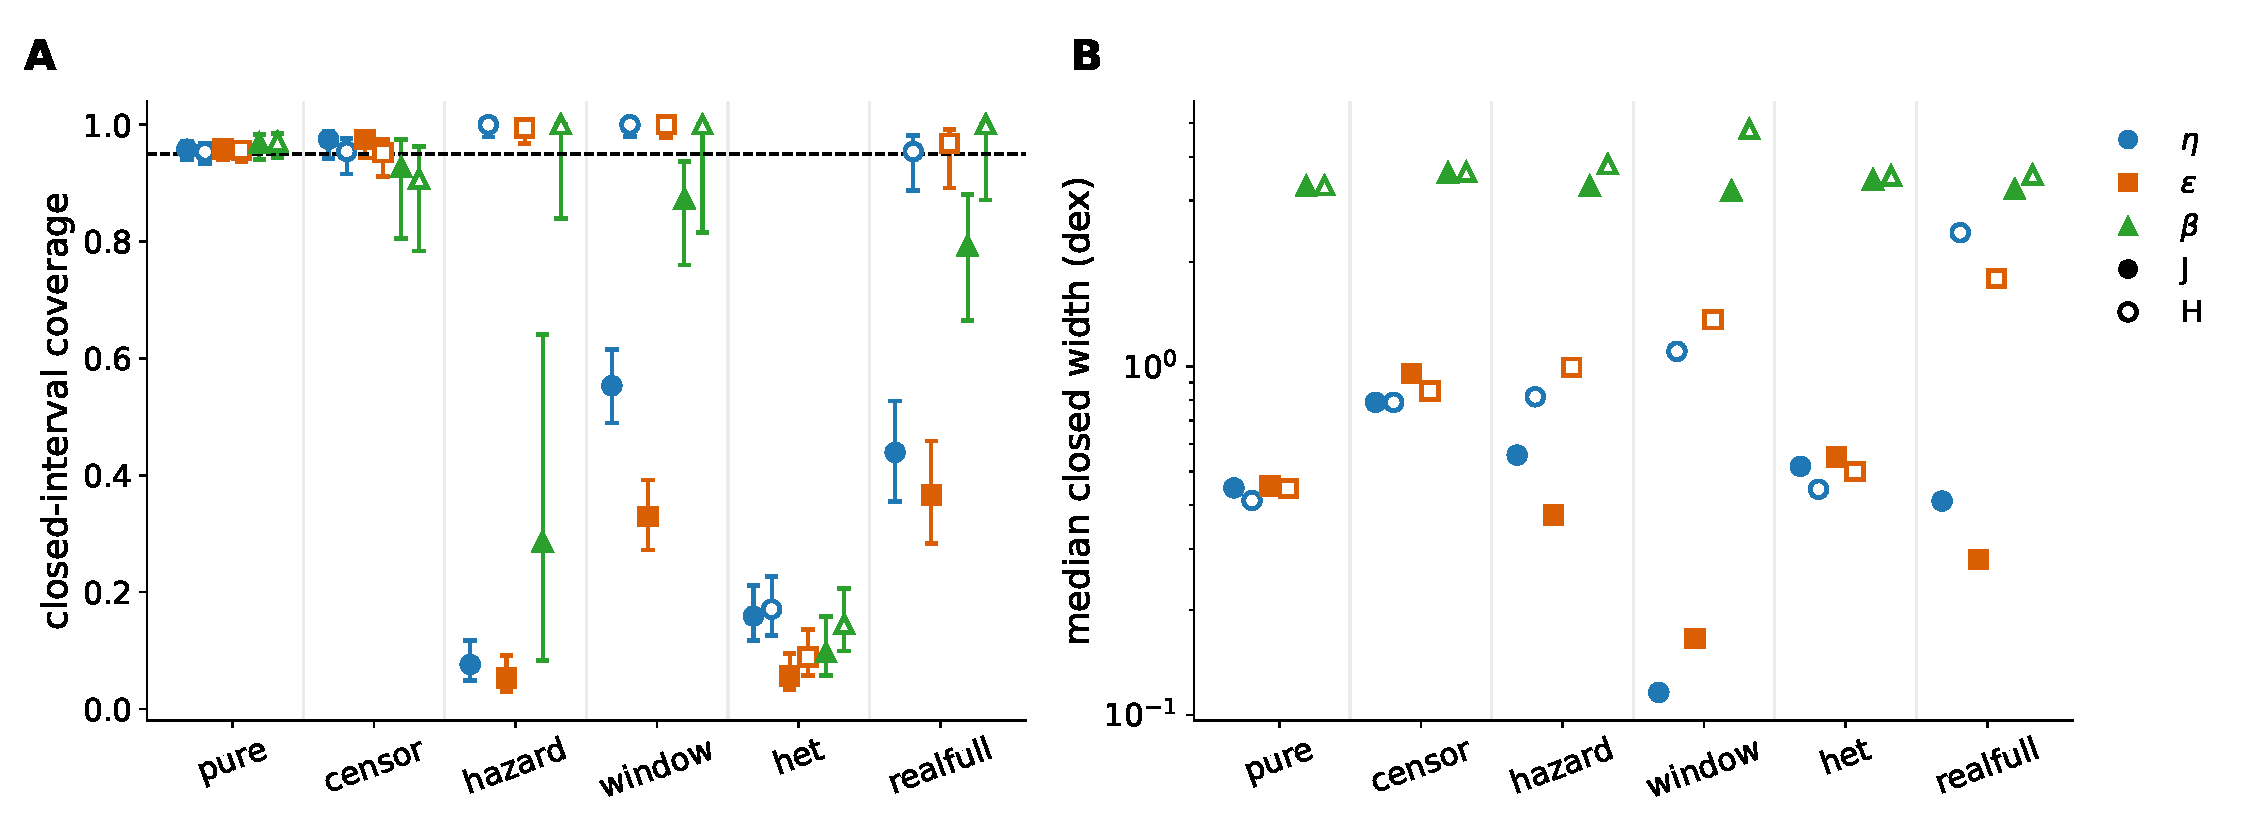
\includegraphics[width=\textwidth]{fig_coverage.pdf}
\caption{Benchmark of the calibrator on library v6 (reference run, \C{gate-v6-n} cohorts). \textbf{A}, closed-interval
coverage of $\eta$, $\eps$ and $\beta$ by arm for J (filled) and H (open); bars are Wilson 95\,\% intervals and the dashed
line is the nominal 0.95. \textbf{B}, median width of the closed intervals (dex, log axis). Arms without closed claims
are omitted; the number of cohorts behind each point is in Table~\ref{tab:coverage-full}.}
\label{fig:coverage}
\end{figure}

\paragraph{Misspecification.} Where the data violate J's assumptions its coverage collapses: on the hazard arm J's closed
$\eta$ intervals contained the truth in \C{v6-hazard-eta-J-hits} of \C{v6-hazard-eta-J-n} cohorts (\C{v6-hazard-eta-J}), and
$\eps$ in \C{d2a-hazard-J-epsilon-coverage}; on the window arm \C{v6-window-eta-J} ($\eta$) and \C{d2a-window-J-epsilon-coverage} ($\eps$). The
variant H, which fits the external hazard and the observation window, restores coverage on these arms: $\eta$
\C{v6-hazard-eta-H} and $\eps$ \C{d2a-hazard-H-epsilon-coverage} (hazard), $\eta$ \C{v6-window-eta-H} and $\eps$ \C{d2a-window-H-epsilon-coverage}
(window), and \C{d2a-realfull-H-eta-coverage} against J's \C{v6-realfull-eta-J} for $\eta$ on realfull. The price is width and
availability: median closed $\eta$ width rises from \C{d2a-hazard-J-eta-median_width_dex} to \C{d2a-hazard-H-eta-median_width_dex} dex (hazard)
and from \C{d2a-window-J-eta-median_width_dex} to \C{d2a-window-H-eta-median_width_dex} dex (window), and H declines $\beta$ on
\C{d2a-hazard-H-beta-decline_rate} (hazard), \C{d2a-window-H-beta-decline_rate} (window) and \C{d2a-realfull-H-beta-decline_rate} (realfull) of cohorts.
Neither variant models a spread of thresholds: on the het arm J's closed $\eta$ coverage is \C{v6-het-eta-J} and H's
\C{v6-het-eta-H}, and both are far below nominal for $\eps$ (\C{d2a-het-J-epsilon-coverage} and \C{d2a-het-H-epsilon-coverage}).
Heterogeneity of this kind is therefore not detected by coverage-based reading of the intervals; it must be checked on
the data (Section~\ref{sec:limitations}).

\paragraph{Windowed fits (W).} W was scored on windowed cohorts of library v6, separately from the reference run above. The
cohorts were split by sample size before the run, at $n=\C{w-large-n}$; the split is the panel's, not a measured change.

\emph{Small and medium cohorts.} The \C{w-a1-n} cohorts with $n<\C{w-large-n}$ were generated at SR parameter grids
(\C{w-a1-n-synth}) or planted at real life tables (\C{w-a1-n-real}, of which \C{w-a1-n-human} human). The closed 95\,\%
intervals of W contained the truth for $\eta$ in \C{w-a1-eta-hits} of \C{w-a1-eta-n} cohorts and for $\eps$ in \C{w-a1-eps-hits}
of \C{w-a1-eps-n}. The cut was fixed before the run, at the coverage that separates a true 0.95 from a true 0.88 given the
number of claims (\C{w-a1-eta-cut} for $\eta$, \C{w-a1-eps-cut} for $\eps$); both were above it. As a second check, the true parameters scored
more than \C{m-chi2-half} nats above W's optimum on \C{w-r3-fail-a1} cohorts. Coverage counts a closed claim whose upper end is
the search box, and such an end cannot miss, so coverage must be read together with the upper ends, below. Where the
data set both ends of the claim, the intervals covered the truth for $\eta$ in \C{w-ends-a1-eta-hits} of \C{w-ends-a1-eta-n}
cohorts and for $\eps$ in \C{w-ends-a1-eps-hits} of \C{w-ends-a1-eps-n}; every $\eta$ miss was a claim with its upper end at the
box, lying above the truth.

\emph{Large cohorts.} The \C{w-a2-n} cohorts with $n\ge\C{w-large-n}$ were synthetic cohorts at human life tables. They give
too few closed claims to tell 0.95 from 0.88, so the pre-registered rule asks only that coverage did not collapse to
\C{w-collapse-level}. Closed intervals covered the truth for $\eta$ in \C{w-a2-eta-hits} of \C{w-a2-eta-n} cohorts (cut
\C{w-a2-eta-cut}) and for $\eps$ in \C{w-a2-eps-hits} of \C{w-a2-eps-n} (cut \C{w-a2-eps-cut}); the rule was met, and the
truth beat W's optimum by more than \C{m-chi2-half} nats on \C{w-r3-fail-a2} cohorts. But the data did not set the upper end
of most closed claims. For $\eta$, \C{w-a2-eta-trunc} of \C{w-a2-eta-n} were truncated above (\C{w-a2-eta-box} at the search
box, \C{w-a2-eta-wid} widened by the profile walk, \C{w-a2-eta-contra} below a point that the walk of the lead pair found inside
the cut), and for $\eps$ \C{w-a2-eps-trunc} of \C{w-a2-eps-n} (\C{w-a2-eps-box} and \C{w-a2-eps-wid}). The pre-registered limit
was \C{w-trunc-max} of the closed claims. It was exceeded, so W warns (\code{W_LARGE_N}) on every windowed fit of
\C{w-large-n} or more rows. Only \C{w-ends-a2-eta-n} of the \C{w-a2-eta-n} closed $\eta$ claims and \C{w-ends-a2-eps-n} of the
\C{w-a2-eps-n} closed $\eps$ claims had both ends set by the data. A widened end is not a limit: the only
$\eta$ miss and the only $\eps$ miss lie \C{w-a2-eta-miss} and \C{w-a2-eps-miss} dex above a widened end. The warning that
follows is that an upper end of a W claim marked box-limited or widened must be read as ``at least this''. The same holds
below the split. In the cohorts planted at real life tables with $n<\C{w-large-n}$, \C{w-a1real-eta-trunc} of
\C{w-a1real-eta-closed} closed $\eta$ claims were truncated above, a share that does not differ from the large cohorts (Fisher
$p=\C{w-fisher}$); for $\eps$ the share was lower, \C{w-a1real-eps-trunc} of \C{w-a1real-eps-closed} against \C{w-a2-eps-trunc} of
\C{w-a2-eps-n} ($p=\C{w-fisher-eps}$). The \C{w-a1-n-human} human cohorts among them, planted at the same life tables as the
large cohorts but with fewer individuals, truncate as the large cohorts do: \C{w-a1h-eta-trunc} of \C{w-a1h-eta-closed} closed
claims for $\eta$ and \C{w-a1h-eps-trunc} of \C{w-a1h-eps-closed} for $\eps$. The life table, not the sample size, sets the
share. Truncated upper ends are common at SR parameter grids too: \C{w-a1syn-eta-trunc} of \C{w-a1syn-eta-closed} closed
$\eta$ claims and \C{w-a1syn-eps-trunc} of \C{w-a1syn-eps-closed} closed $\eps$ claims.

The ratio $\eta/\eps$ closes where $\eta$ alone does not. The combinations were scored on one cohort per cluster. On the small
and medium cohorts $\eta/\eps$ was closed on all \C{w-lead-a1-ee-n} and covered the truth on \C{w-lead-a1-ee-hits};
$\beta\rbar/\eta$ was closed on \C{w-lead-a1-re-n} (covering \C{w-lead-a1-re-hits}) and was an upper bound on
\C{w-lead-a1-re-os-n}, all of which covered. On the large cohorts both were closed and covered the truth, on
\C{w-lead-a2-ee-hits} of \C{w-lead-a2-ee-n} and \C{w-lead-a2-re-hits} of \C{w-lead-a2-re-n}; these counts are too small to
show 0.95.

\emph{Cohorts at real data sets.} The \C{w-rf-n} cohorts of the realfull arm (\C{w-rf-n-human} human, \C{w-rf-n-fly}
Drosophila) are not real data in the sense of an unknown truth. Each is generated from the SR model at parameters fitted to a
real data set, on that data set's window, at a design sample size from \C{w-rf-fly-nmin} to \C{w-rf-nmax} (on the four cohorts of
one fly data set the window removes no record). Each is therefore scored against the parameters that generated it, and the arm
is reported, not gated. Closed intervals covered the truth for
$\eta$ in \C{w-rf-eta-hits} of \C{w-rf-eta-n} and for $\eps$ in \C{w-rf-eps-hits} of \C{w-rf-eps-n}. Yet \C{w-rf-eta-trunc} of the
\C{w-rf-eta-n} closed $\eta$ intervals and \C{w-rf-eps-trunc} of the \C{w-rf-eps-n} closed $\eps$ intervals were truncated above. The
data set the upper end of $\eta$ on \C{w-rf-eta-cap} of the \C{w-rf-n} cohorts and of $\eps$ on \C{w-rf-eps-cap}.

\emph{Is the reported optimum the best point?} J keeps its optimum when a profile walk finds a better point by less than
\C{m-chi2-half} nats, so the reported optimum can lie below the best point the fit saw. A pre-registered rule asked that W's
optimum score within \C{w-opt-tol} nats of the best point of H's fit with the smallest hazard, and its stated consequence on
failure was to withhold W. It failed, on \C{w-opt-a1-fail} of \C{w-a1-n} small and medium cohorts (largest gap
\C{w-opt-a1-max} nats), \C{w-opt-a2-fail} of \C{w-a2-n} large cohorts (\C{w-opt-a2-max}) and \C{w-opt-rf-fail} of \C{w-rf-n}
realfull cohorts (\C{w-opt-rf-max}). We waived the consequence after seeing the result: every gap was below \C{m-chi2-half}
nats, so the claims, which are widened to include the best point, still contain it; the truth never scored more than
\C{m-chi2-half} nats above W's optimum; and a refit of one failing cohort per group found a gap of the same size. The window makes the
gap more frequent. Of the \C{w-opt-syn-n} cohorts at SR parameter grids, W's gap (to H's fit at the smallest hazard) exceeded
\C{w-opt-tol} nats on \C{w-opt-syn-w}, and J's gap (to the best point of its own fit), on its stored fit of the unwindowed twin of
the same cohort, on \C{w-opt-syn-j} (Fisher $p=\C{w-opt-syn-p}$); the two gaps are measured from different reference points.
The optimum also depends on the machine on a human-size cohort. The refits above were made on a second computer, one per
group ($n=\C{w-host-a1-n}$, \C{w-host-realfull-n} and \C{w-host-a2-n}). On the two non-human cohorts they matched the first
computer to within \C{w-host-other-max} nats. On the human cohort the second computer found a log-likelihood \C{w-host-ll}
nats better, with $\eta$ \C{w-host-eta}\,\% and $\kappa$ a factor \C{w-host-kappa} apart. All \C{w-host-in} of
\C{w-host-nref} refitted optima lay inside the first computer's claims; the second computer's own claims were not recorded.
Report the claims of W, not its point estimate.

\emph{Leverage.} The drop-one leverage check (Section~\ref{sec:val-leverage}) raised
\C{w-lev-flags} flags on the \C{w-lev-assessed} W fits it could assess, when nothing was planted, of which \C{w-lev-slides}
were flat-valley slides. It could not assess \C{w-lev-notass} of the \C{w-lev-human-n} fits at human life tables. Its
detection on windows was not tested.

\paragraph{Sharp cohorts and the $n$-ladder.} On the \C{d2a-sharp-pure-valid-n} valid sharp pure cohorts J's closed $\eta$ intervals
contained the truth in \C{d2a-sharp-pure-eta-hits} of \C{d2a-sharp-pure-eta-n} (\C{v6-sharp-pure-eta-J}); the
flagged sharp cohorts form a defect panel and are not scored as coverage. On the $n$-ladder (\C{v6-group-nladder} pure
cohorts at all $\kappa$ values and $n$ between \C{v6-n-min} and \C{d2a-nladder-n-max}) closed $\eta$ coverage was
\C{v6-nladder-eta-J} (\C{d2a-nladder-eta-hits} of \C{d2a-nladder-eta-n}) and closed $\eps$ coverage \C{v6-nladder-eps-J}
(\C{d2a-nladder-eps-hits} of \C{d2a-nladder-eps-n}). Coverage thus stays near nominal across sample sizes; the cost of
small $n$ and sharp death ages is width, not miscoverage.
The variant H was not run on these two groups, so its coverage there is not known
(Section~\ref{sec:limitations}).

\paragraph{One-sided bounds.} When a closed interval is not available the calibrator may still claim a bound.
Pooled over all arms of the reference run (\C{gate-v6-n} cohorts; \emph{not} per arm), J's one-sided claims cover the
truth for $\eta$ in \C{d2a-J-onesided-eta} of cases, $\eps$ in \C{d2a-J-onesided-epsilon}, $\beta$ in \C{v6-J-onesided-beta} and
$\kappa$ in only \C{v6-J-onesided-kappa} (\C{d2a-J-onesided-kappa-hits} of \C{d2a-J-onesided-kappa-claimed} bounds), against
\C{v6-H-onesided-eta}, \C{v6-H-onesided-epsilon}, \C{v6-H-onesided-beta} and \C{v6-H-onesided-kappa} for H. J declines $\kappa$ in
\C{v6-J-kappa-declined-frac} of cohorts. These bounds are not reliable for J on misspecified arms, and $\kappa$ and
raw $\beta$ should not be reported as estimates (Section~\ref{sec:identifiability}).

\paragraph{Cost.} A J fit took a median of \C{cost-J-median-cpu} CPU-seconds per cohort and the J reference run
\C{cost-J-total-cpuh} CPU-hours in total; the H run took \C{cost-H-total-cpuh} CPU-hours, a median per-cohort ratio of
\C{cost-H-over-J}. The J fits ran on five processor models (\C{gate-v6-offref-records} of \C{gate-v6-n} records off the
reference model; Section~\ref{sec:software}).
